\chapter{Evolution of PWAs and capabilities}

\section{Smartphones are everywhere}

The smartphone has seen an incredible rise in ubiquity since its inception. What could once be done only with an expensive desktop computer with a multitude of peripherals, is now available on a comparatively cheap mobile device.

Plotting market shares of desktop, mobile and tablet devices against one another, like shown in Figure \ref{FigStatCounterDMT}, it is easy to notice how mobile devices have slowly overtaken desktop devices in popularity in the last 15 years.

\begin{figure}[htbp]
    \centering
    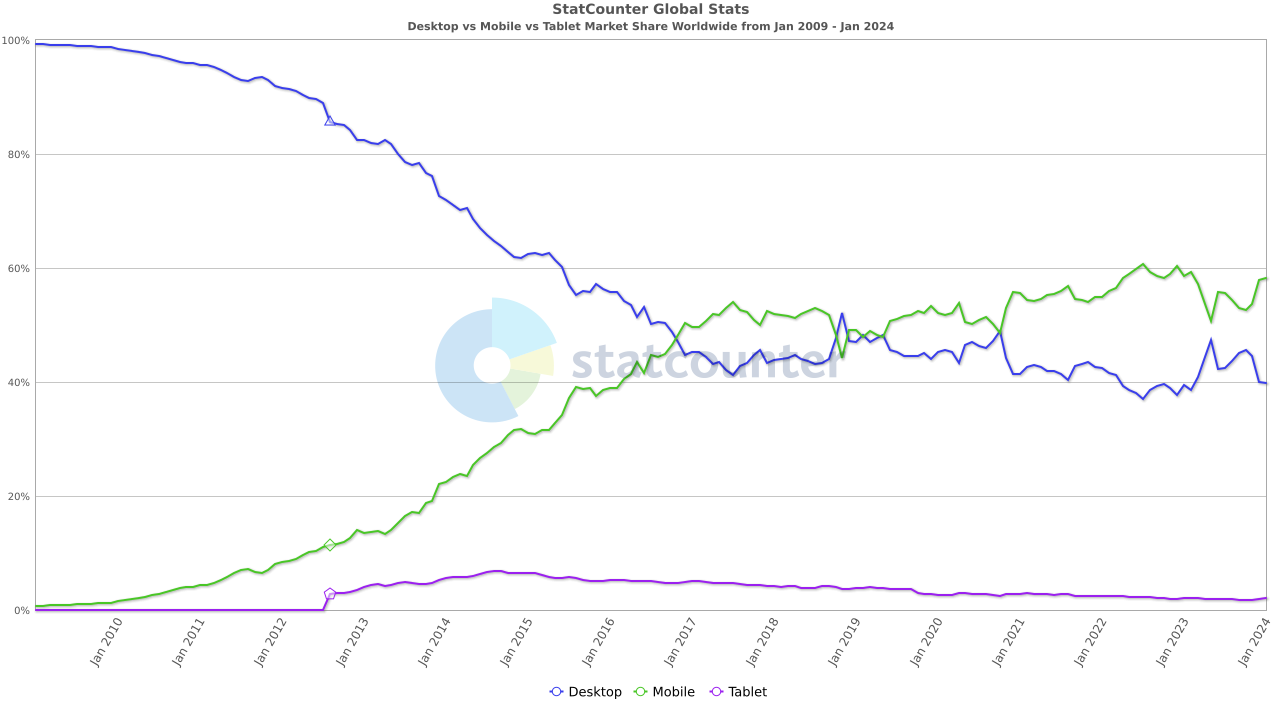
\includegraphics[width=\textwidth]{./figures/ch2_desktop-vs-mobile.png}
    \caption{Market shares of desktop, mobile and tablet devices, from January 2009 to January 2024 \cite{StatCountDMT}. Starting August 1st 2012, the chart counts tablets as a separate metric.}
    \label{FigStatCounterDMT}
\end{figure}

The trend of owning a mobile device shows that people prefer carrying a small and capable device around, rather than only being able to connect to the Internet using their fixed and comparatively large desktop device.

\section{Design differences and similarities between desktop and mobile}

\subsection{Evolution of desktop devices}

It is worth noticing that these two platforms could not be more similar to one another, yet have so many differences. Desktop devices have a notably different evolutionary tree to mobile devices, which means that not only do their shapes and buttons differ, but also their design philosophies.

Computers in their earliest forms were generally thought of as "boiler-room infrastructure" rather than personal devices. The advent of devices like the Apple II and software like VisiCalc, which was an advanced-for-the-time spreadsheet processor released in 1979, started to prove to the world that computers are not only useful when used by a trained team of experts, but can automatize tasks in the reach of a single employee \cite{NYBirthPC}.

These flashy, almost magical machines were starting to be capable of doing various tasks, from boring data processing to running graphics and games. This, combined with how they started to become more and more affordable, resulted in a boom in personal computer ownership starting in the 1980s.

\begin{figure}[htbp]
    \centering
    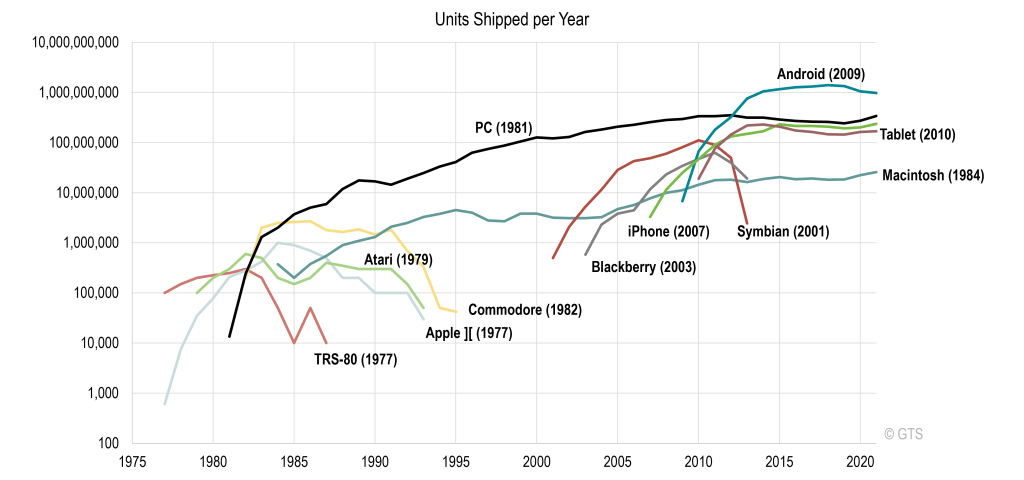
\includegraphics[width=\textwidth]{./figures/ch2_historical_pc_usage.png}
    \caption{Units Shipped per year for various desktop PCs and mobile devices, from 1977 to 2021 \cite{TGPCHis}.}
    \label{FigHistoricalPC}
\end{figure}

This direct lineage between the personal computer and pre-1970 mainframes is apparent in the architectures of common operating systems like Windows or Unix. Given how specialized machines, that required trained people to use, started to spread to less technically advanced end-users, it is understandable that computer and operating system vendors tried to simplify how their systems were used.

In particular, the Personal Computer (PC) developed by IBM has seen the longest lifetime of a single lineage of computers (Figure \ref{FigHistoricalPC}), being traceable all the way from 1981 to today. This shows that the evolution of the IBM PC occurred in incremental steps, and to avoid having software vendors be forced to upgrade their software upon release of every version, it is understandable that IBM offered a degree of backwards compatibility.

As a result, design decisions that made sense in the 1980s started to be less useful. A notable example of such design decisions can be found in modern Windows operating systems. The Microsoft documentation \cite{MSDNFolderNaming} has a clause that specifies a number of disallowed directory and file names, the likes of "CON", "PRN", "NUL", "AUX", and others, in addition to any combination of these names with any extension. This is very likely a result of the desire to keep backwards compatibility with old MS-DOS systems, that Windows can be directly traced to, which used these names as aliases for device drivers \cite{HusseinDeviceDrivers}.

\subsection{Evolution of mobile devices}
In comparison, the evolution of mobile devices and smartphones is very distinct and contained in a much shorter period of time.

The first device that was described as "the first time someone created a computer into the shape of a phone" is credited to be the IBM Simon, released around 1992. Boasting a touch screen and being portable, it had features such as a calculator and email. It has been described, retroactively, as "[being] the first smartphone. Twenty years ago, it envisioned our app-happy mobile lives, squeezing the features of a cell phone, pager, fax machine, and computer into an 18-ounce black brick"
\cite{SagerIraHistoryOfPhones}.

The year 1992 is very recent, compared to when the first computers started to become mainstream. This allowed phone manufacturers and OS vendors to learn from the mistakes done by personal computers, or optimize certain user experience facets.

An important step in the evolution of mobile devices is widely regarded as being the first iPhone. The hype Apple created about their new and flashy smartphone, culminating in around 11.000 print articles and 69 million hits on Google, seems to have been justified, and the phone was revolutionary, although somewhat flawed \cite{NYTAppleIPhoneRelease}. The iPhone defined a new era of smartphones, and many phone manufacturers have followed in the path that Apple laid out.

One of the core ideals of the iPhone is the ease of use. People that are non-technical find the iPhone accessible, and the way it seamlessly integrates with other Apple (sadly, only Apple) products proves that technology does not necessarily have to be hard to use \cite{SlashGearIPhoneOverAndroid}.

This trend manifests itself across the entire range of available mobile devices versus personal computers. Mobile phones are more widespread and are generally easier to use, having more friendly user interfaces and abstracting away hard technical details as much as possible.

\section{Native applications}

Mobile devices present ways of installing additional programs called "applications" that can extend the functionality of the device. Applications have proven to be the de-facto standard for implementing mobile functionality, and an ever-increasing number of companies offer their services through the apps that they constantly ask consumers to install.

From an architectural standpoint, these applications are strongly tied to the operating system architecture, and are therefore not portable.

Having said that, an attempt at portability and standardization across mobile devices can be found within the Android Open Source Project. An initiative by Google, the project offers a full mobile operating system under an open-source license, thus allowing any phone maker across the world to use it as a starting point for their own operating system.


\section{Hybrid (cross-platform interpreted) applications}

\section{Web applications}

\section{Progressive Web Apps}

\section{Comparison}